%!TEX root = proj_report_outline.tex
\chapter{Experiment Design and Test Bed}
Following the completion and deployment of the prototype, an analysis of the artefacts produced was carried out. The evaluation was designed to verify the successfulness of the project against the requirements identified in Chapter \ref{C:requirements}. To build confidence in the results derived, this chapter discusses the scope, assumptions, and limitations as well as the design of the experiments themselves.

\section{Evaluation Scope}\label{S:evaluationScope}
In designing the evaluation, the requirements identified in Chapter \ref{C:requirements} were deconstructed to clearly define, where possible, the conditions upon which each requirement can be considered fulfilled. The high-level results of this requirements deconstruction is displayed in the following table:

\begin{table}[h!]
\begin{adjustwidth}{-1.25cm}{}
\begin{tabular}{ |p{1cm}||p{6cm}|p{10cm}|  }
 \hline
 ID & Requirement & Fulfilment Criteria\\
 \hline
    D1 & Enable the innovation community to collaborate & 1. User stories describing collaboration in the innovation 
  community are specified\newline2. These user stories specified are supported\\
 \hline
    D2.1 & Enable users to scope the disclosure of their content/identity & 1. User stories describing content/identity scoping are specified\newline2. These user stories specified are supported\\
 \hline
    D2.2 & Provide auditing functionality & 1. User stories describing auditing are specified\newline2. These user stories specified are supported\\
 \hline
    D2.3 & Store sensitive data securely & 1. A security expert verified the system\\
 \hline
    D3 & Be portable and extensible & 1. Discern from requirements\\
 \hline
    D4 & Be performant & 1. Measure(s) of performance are defined\newline2. These measures are met\\
 \hline
    D5 & Support a distributed architecture & 1. A distributed system is designed and implemented\\
 \hline
\end{tabular}
\caption{A breakdown of the requirements and their corresponding fulfilment criteria.}
\label{Table:innovation_breakdown}
\end{adjustwidth}
\end{table}
\vspace{1em}

Requirements D1, D2.1 and D2.2 have very similar fulfilment criteria and hence have been grouped together for the evaluation. Through this evaluation it is established that PitchHub has the required functionality to support collaboration within the innovation community. The experiment design and test bed implemented for these functional requirements are described in Section \ref{SS:collaborativeFunctionality}.

Requirement D4 relies on a simulation based evaluation, where synthetic data is seeded to imitate the load the entire innovation community in New Zealand would have on PitchHub. Requirement D5 is implicitly satisfied through this experiment as the simulation is deployed on distributed infrastructure. Through this experiment it is established that the PitchHub application has the ability to support the innovation community. The experiment design and test bed implemented for these non-functional requirements are described in Section \ref{SS:performance}.

Table \ref{Table:innovation_breakdown}'s fulfilment criteria denotes the steps required to satisfactorily mark the requirement as completed, and as seen in requirement D2.3 and D3 some of these steps require external review. The implications of this are now discussed.

Achieving a conclusive degree of verification for requirement D2.3 would require a level of scrutiny and knowledge possessed only by security experts. An evaluation of this requirement would require consideration of the following points: first, the cryptographic modules in the Secret Sharing Service must be verified and second, the security of the storage functionality could not be performed in isolation. Should any combination of access control, communications, or session management components be compromised it is possible that the storage functionality component may also be compromised by association. Therefore evaluating whether ``data is stored securely'' must be done within the context of the wider system rather than specifically on the Secret Sharing service. Verifying the Secret Sharing service's cryptographic implementation would take us further down the rabbit hole. OWASP's application security verification standard \cite{OWASP:online} details the minimum standard: all cryptographic modules fail securely, random number generators apply the appropriate standards, all cryptographic modules are validated against FIPS 140-2 or equivalent, and all cryptographic modules operate in their approved mode according to their published security policies. Given the large burden to validate this requirement and the project's limited resources I regard the verification of requirement D2.3 out of scope. Cursory steps I have taken to build confidence in the prototype's security are as follows: implementation of a Shamir's Secret Sharing service, all requests enforce ssl, CSRF tokens to prevent CSRF, escaped user input to prevent XSS, 
white-list firewall set-up, \textit{fstab} modification to prevent shared memory attacks, \textit{sysctl} and host file modification to prevent IP Spoofing, and DenyHosts \cite{DenyH6:online} integrated to prevent SSH attacks.

Assessing whether a system is portable and extensible is inherently subjective. The fulfilment criteria for requirement D3 reflects this. A system could be regarded as portable if it works in all environments required of it, and likewise a system could be regarded as extensible given it is able to adapt to all it's future requirements. However, determining all the future environments and requirements of the system is a difficult task. PitchHub has therefore sought to achieve general portability and extensibility. The definition of portability adopted is: ``the ease with which a system or component can be transferred from one hardware or software environment to another'' \cite{mattsson2006software}. As discussed in previous sections PitchHub has employed virtualisation and automation to make such tasks easy as possible. The definition of extensibility adopted is: ``the ability of the system to tolerate additional features or functionality will little or no required rework of previously developed features or functions'' \cite{Extensibility:online}. PitchHub has been developed with this in mind, the layered architecture and MVC pattern followed mean that both hardware and software components are divided in terms of responsibility. This separation of concerns means that future change request modifications will be isolated to components whose responsibility fits. The inability to strictly quantify or qualify whether requirement D3 is met has led me to regard this requirement as out of scope for the purposes of this evaluation. However I believe the spirit of this requirement has been reflected in the system's design.

\section{Assumptions and Limitations}
The experiments undertaken have operated under a number of assumptions and limitations. These assumptions and limitations are explored in this section. Reflection on these assumptions and limitations are provided with discussion on their possible ramifications.

A limitation of the experiment described in Section \ref{SS:performance} is that it is seeded with synthetic data rather than user data. This is because no open-source user data currently exists within the domain of collaborative innovation networks\footnote{As of 29/9/15.}. To achieve a representative synthetic dataset I required: the number of people in the innovation community (to determine user base size), and also an idea of their platform engagement (to determine a distribution of the PitchCards contributed). Statistics New Zealand's (SNZ) data on innovation activities in New Zealand gives a picture of the innovation communities size from 2003 to 2013 \cite{Innov5:online}. 
SNZ's data is based on the population of businesses in New Zealand who categorise themselves as participating in ``innovation activity''. An important feature to note is that the data does not feature sole traders or businesses with less than 6 employees. SNZ's data categorises New Zealand businesses by size (e.g. 6 - 9 people, ... 50 - 99 people) and maps how many companies fit each range. 
This data presents three concerns: first, the small businesses not included may represent an appreciable portion of PitchHub's target audience. Second, the large ranges provided lowers the fidelity of the results derived. Third, by using the total business size the SNZ data includes people who do not directly have a stake in the innovation ecosystem (i.e. not resembling one of the roles identified in Section \ref{background}). These limitations have been deemed acceptable for the purposes of this evaluation because the goal is merely to build confidence that the prototype could work in production. Ultimately, this data gives a ballpark, albeit overly high, estimate of the size of the innovation community in New Zealand. The results from this analysis is presented in Table \ref{tab:title} and Figure \ref{fig:innovation_size}.

\begin {table}[H]
\begin{center}
\begin{tabular}{ |p{2cm}||p{3cm}|p{3cm}|  }
 \hline
 \multicolumn{3}{|c|}{Estimated total number of employees of businesses}\\
 \multicolumn{3}{|c|}{with innovation activities from the years 2005 to 2013} \\
 \hline
 Year & Expected Size & Worst Case Size\\
 \hline
    2005 & 453,619.5 & 613,929\\
 \hline
    2007 & 454,365 & 615,068\\
 \hline
    2009 & 431,442 & 578,196\\
 \hline
    2011 & 416,065.5 & 559,959\\
 \hline
    2013 & 431,524.5 & 579,549\\
 \hline
\end{tabular}
\end{center}
\caption {Estimates of total number of employees in businesses with innovation activities derived from Statistics NZ data.} \label{tab:title} 
\end {table}

\begin{figure}[ht]
    \centering
    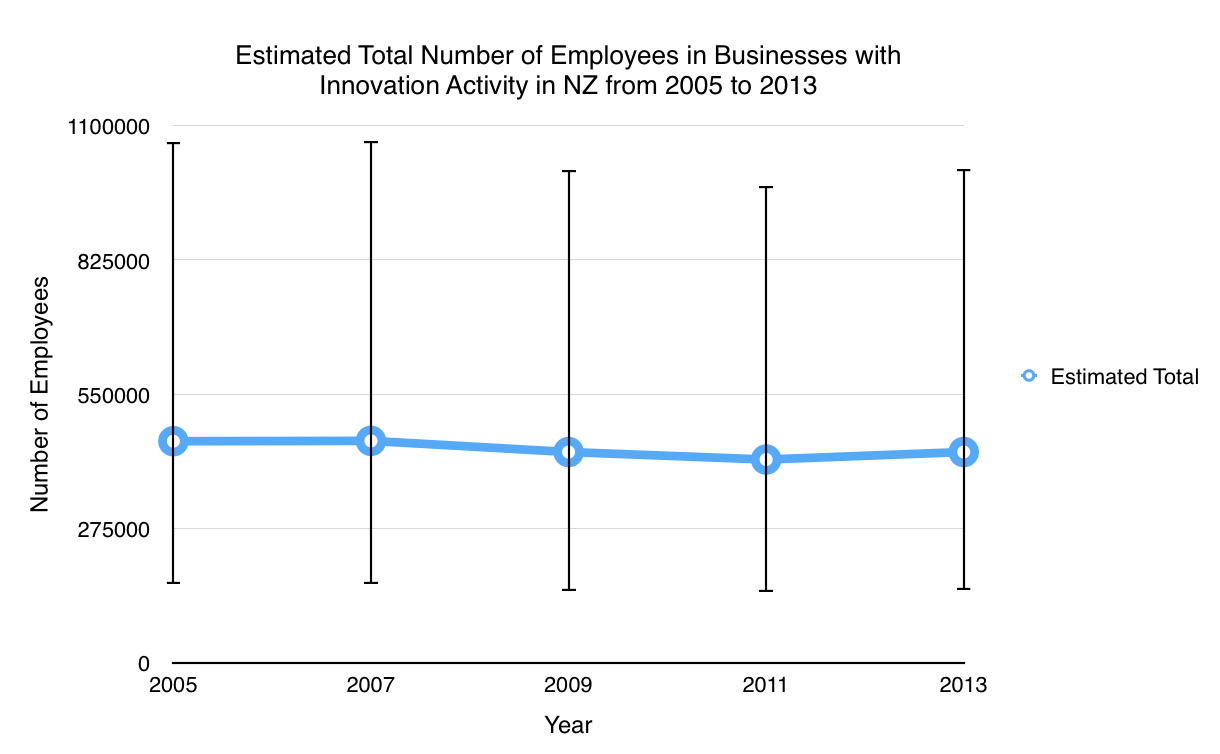
\includegraphics[width=0.7\textwidth]{innovation_size}
    \caption{The estimated total number of employees in businesses with innovation activities from the years 2005 to 2013. The disparity between the expected sizes vs. worst case sizes is resultant from the wide range presented in the data.}
    \label{fig:innovation_size}
\end{figure}

The results shown identify the expected estimated size of the innovation community as well as the worst case estimated size (calculated using the upper range). The figures presented are believed to be quite high given that the current total workforce population of NZ is estimated to be 2.3 million people \cite{WorkingPopulation:online}. These figures being high however further build confidence that the prototype can support the NZ innovation community.

An informed estimation of the amount of contributions each user may have is inherently important to a performance evaluation where database queries make up the majority of processing time. To make the seed data more realistic a Pareto distribution, Figure \ref{fig:contribution_distribution}, was chosen with Callaghan Innovation. The reason for such a distribution is that we conjecture that the vast majority of users will likely make only a few Pitch Cards and Suggestions, while a long tail of more avid users will be contributing a disproportionate amount of Pitch Cards and Suggestions relative to the entire user base. This conjecture is supported by recent work analysing user engagement in online support groups \cite{carron2014describing}\cite{van2015mapping}. The authors of both papers find that similar power distributions are able to characterise user engagement.

\begin{figure}[ht]
    \centering
    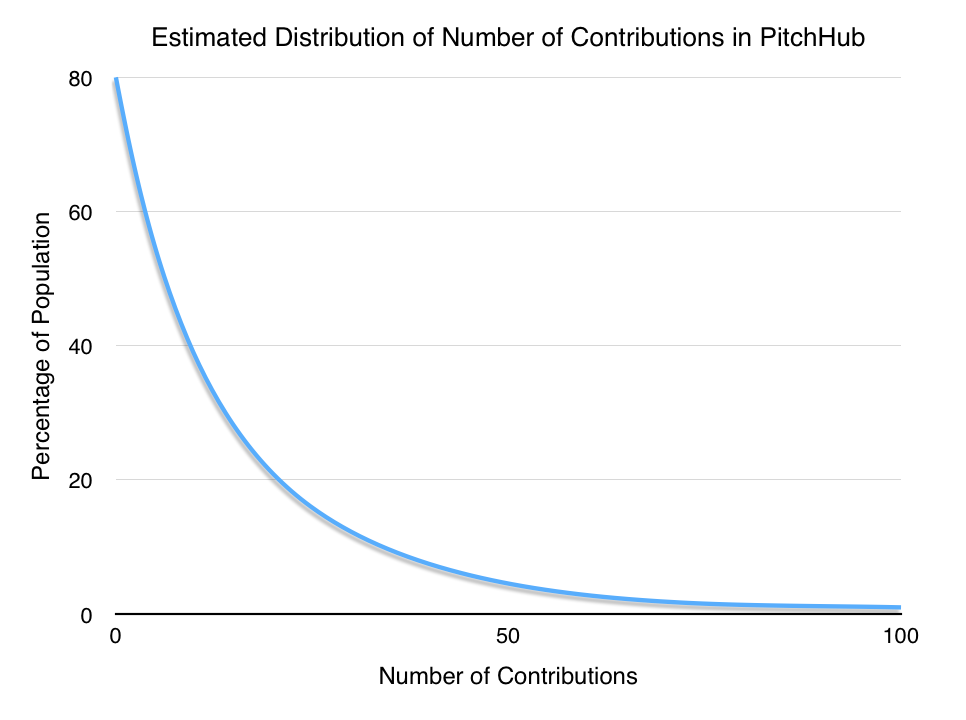
\includegraphics[width=0.7\textwidth]{contribution_distribution}
    \caption{The assumed Pareto distribution describing user engagement with regard to Pitch Cards and Suggestions shared.}
    \label{fig:contribution_distribution}
\end{figure}

One of the key assumptions underpinning the PitchHub system is that the functionality specified in the user stories will actually facilitate collaboration within the innovation ecosystem. There has been no prior user study nor previous works which indicate that the collaborative approaches embraced (idea-deconstruction/scope of disclosure) by the prototype will either help or hinder the collaboration process. Based on Callaghan Innovation's experience in the innovation community and the current trend of platforms being released targeting innovators (e.g. IdeaForge and Assembly identified in Section \ref{background}) we believe that there is an inherent need for online collaboration within this community. Ultimately, discerning whether the prototype produced has the ability to satisfy this need will be determined through experience. Currently the prototype has been bought into by the wider Callaghan Innovation networks group. This is an ideal \textit{proving ground}, as it means that resources will be made available to continue PitchHub. Furthermore, the acceptance by a separate Callaghan Innovation group is a positive indication that the functionality supported is desired.

A limitation of the experiment design for the functional testing is that Selenium uses Firefox. Online sources agree that Google Chrome holds the dominating market share of browser usage at around 60\%, as opposed to Firefox's share at around 20\% \cite{Brows6:online}. Ideally, simulations would be run on all major browsers but as it stands the Firefox driver for Selenium is the most robust and complete. However, this limitation is considered to be acceptable given that browser vendor conformance to W3C standards is high \cite{WebB1:online}.

\section{Test Design}
This section explores the three test beds designed for the evaluation. Each test bed was designed with different responsibilities in mind. The first, \textit{TB1}, evaluates the collaboration functionality supported for requirements D1, D2.1 and D2.2 using `executable' user stories. The second, \textit{TB2}, evaluates the the prototypes performance in various distribution configurations for requirements D4 and D5. The third, \textit{TB3}, evaluates the collaboration functionality supported for requirements D1, D2.1 and D2.2 using a live deployment and real users. The design and aim of each test bed is discussed with reflection on how automation has also been used to improve their flexibility.

\subsection{Test Bed 1 - Collaboration Functionality}\label{SS:collaborativeFunctionality}
The principal aim in testing the fulfilment of requirements D1, D2.1 and D2.2 is to ensure that users have the tools/functionality available to successfully collaborate online. Specifically what successful online collaboration is, has been captured in the user stories developed by Callaghan Innovation and myself. The following is an example (concatenated for brevity) of the general granularity achieved in each `executable' user story:

\begin{lstlisting}[language=ustory,firstnumber=1]
Feature: Annotate Pitch Card
  As a user, I want to suggest changes on viewable pitches so that I can offer insight

  Background:
    Given following users exist:
      | username    | email             |
      | Foo         | foo@foo.foo       |
      | Bar         | bar@bar.bar       |
    And a user with email "foo@foo.foo" posts a well formed pitch card

  Scenario: suggest a change
    When I sign in as "bar@bar.bar"
    And I am on the first pitch card contributed by "foo@foo.foo"
    And I click "suggest" on the pitch point "solve"
    And I fill in the following:
      | change              | my suggested change                   |
      | comment             | reasoning for my change suggestion    |
    And I set the content scope of disclosure to "public"
    And I set my identity scope of disclosure to "collaborators"
    And I press "Submit"
    Then I should see "my suggested change" within "discourses-content"
    And I should see "reasoning for my change suggestion" within "discourses-content"
    And I should see "less than a minute ago" within "discourses-content"

\end{lstlisting}

The test bed PitchHub uses for evaluating the functional requirements, \textit{TB1}, `executes' these user stories. It does so in exactly the same way users interact with the system, through a browser. This has been achieved by using Cucumber, a Ruby behaviour driven development library, and Selenium, a popular web driver.

To demonstrate how these `executable' user stories sufficiently simulate user behaviour the above example is considered. The feature \textit{Annotate Pitch Card} contains three main sections: a brief description of the test's aim, the background which specifies the beginning state of each test, and scenarios which are essentially the feature's tests. The content of the background and scenario blocks are interpreted via step definitions which use Selenium to then drive browser interaction (clicks, text input, etc.). For example, the line ``When I sign in as bar@bar.bar'' is interpreted through the step definitions into the following browser interactions: navigate to page \url{localhost:3000/users/sign_in}, fill email field, fill password field, click login button.
A key advantage in having functionality testing automated in this way is that the state of the application is far simpler to reason about. At the start of each test the application is guaranteed to always be in the state specified in the background and throughout each scenario all statements following the `then' keyword act as assert statements making in-test guarantees possible.

Ultimately, the aim of ensuring functionality is supported, is well-suited to this type of testing for the following reasons: first, user interaction is simulated naturally, second, automation ensures that no lingering tests and their leftover states affect current tests, and third, the natural definition of these tests mean that non-technical users can specify and test behaviour.

\subsection{Test Bed 2 - Performance}\label{SS:performance}

In evaluating performance there are a number of metrics that may be analysed e.g. latency, throughput, capacity. Ultimately, the wall-time metric was chosen because it reflects the performance of the system as experienced by the user. As PitchHub is a user-facing applications this was deemed to be the most important measure. To determine the prototype's fulfilment of requirements D4 and D5 the average wall-time to process a request in the various configurations is evaluated. Wall-time is a key metric on which to evaluate performance as it represents the request's end-to-end processing time. This means that the time taken for server-side processing, database queries, and client-side processing are included in the results. This test bed, \textit{TB2}, is used for several experiments: comparing the performance under different user base sizes, testing the overhead added through diverse secret keepers, and testing the overhead added of the Secret Sharing scheme. Common amongst the tests is that they rely on the authenticity of the configuration/data used to derive meaningful results. To create an authentic test bed and environment several steps were taken:
\begin{itemize}  
    \item The application is hosted on a Passenger application server with production settings (e.g. caching).
    \item The tests simulate user input via the REST API.
    \item The user base sizes are modelled off of the Statistics New Zealand innovation reports.
    \item The infrastructure used reflects a highly available production configuration, see Figure \ref{fig:architecture_evaluation}.
\end{itemize}

\begin{figure}[ht]
    \centering
    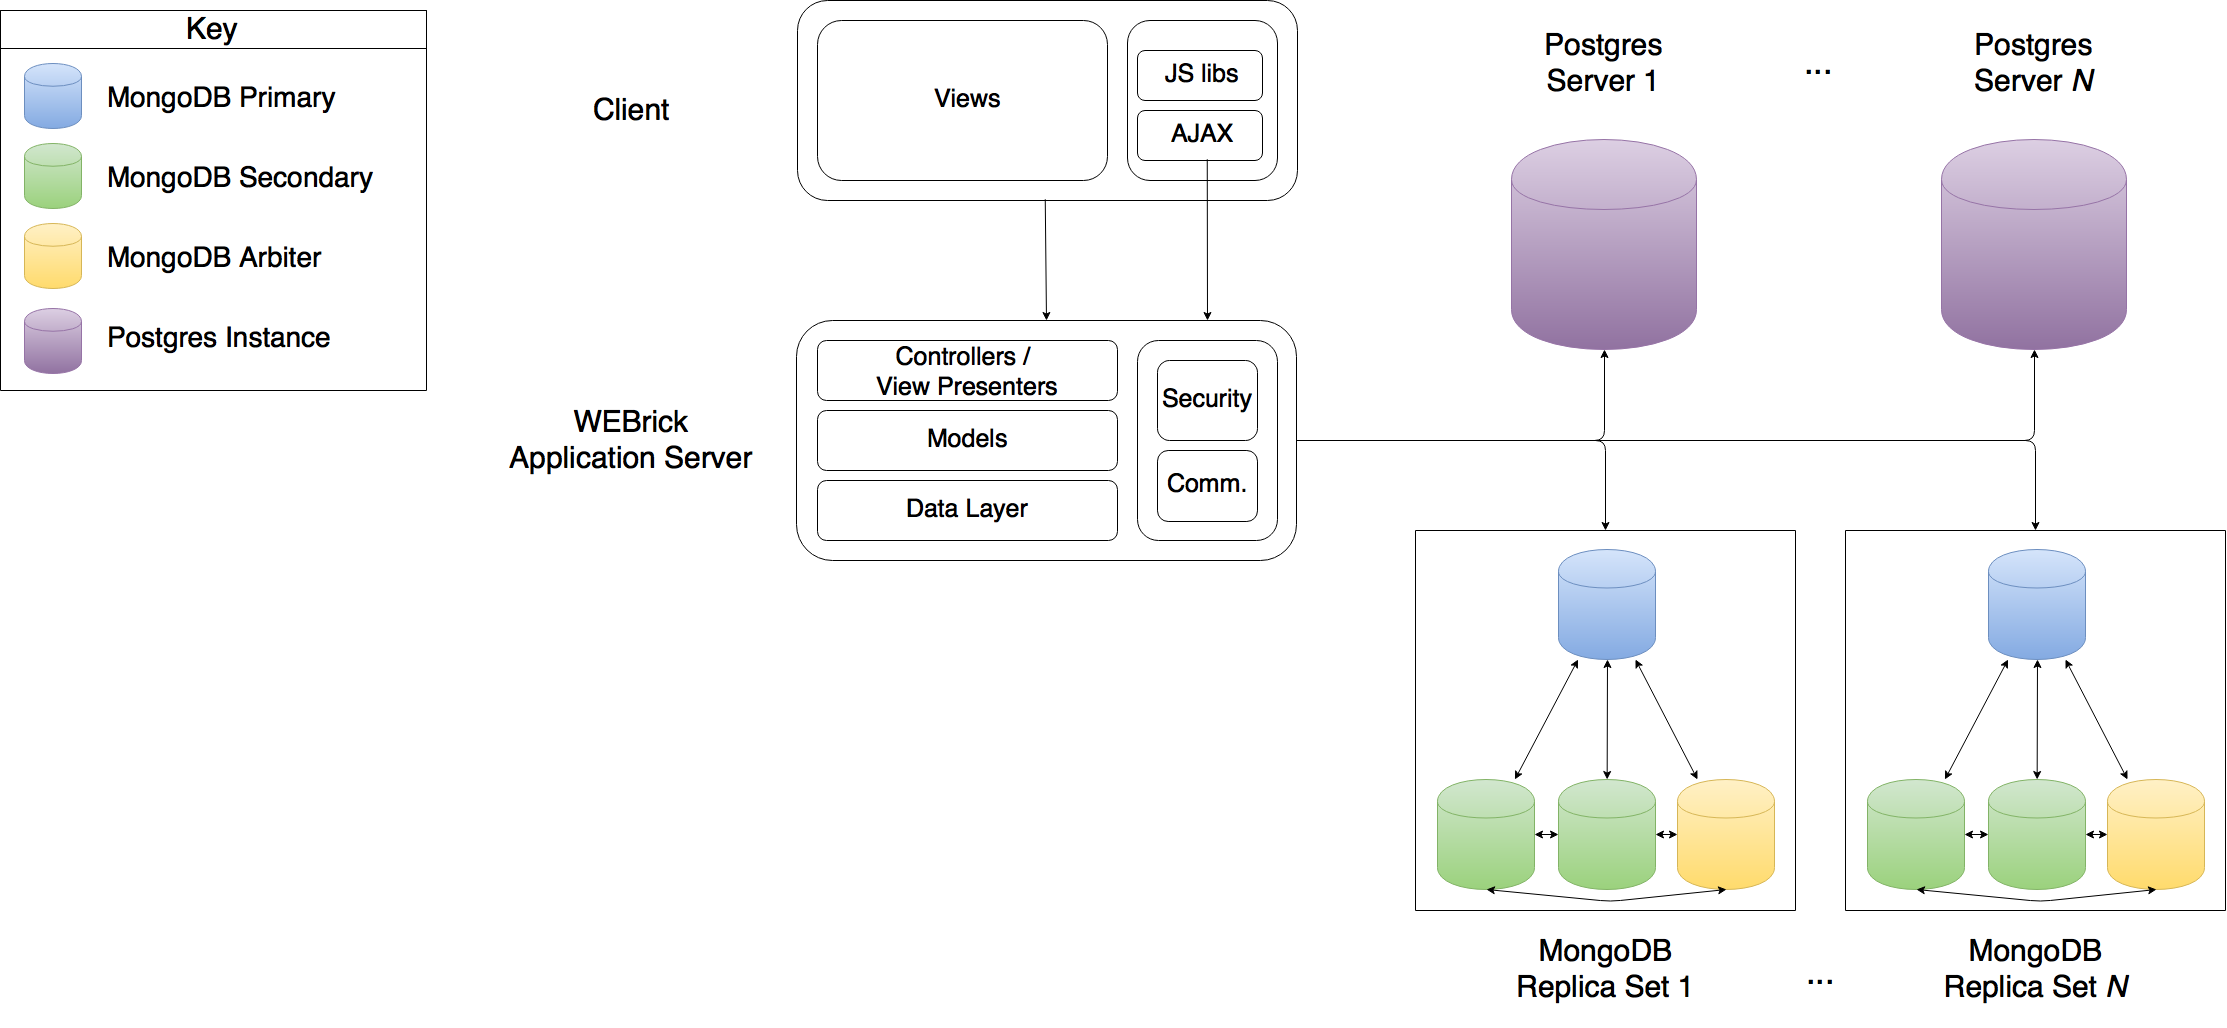
\includegraphics[width=1\textwidth]{evaluation_architecture}
    \caption{The architecture used for \textit{TB2}. The MongoDB secret keepers are replica sets, the redundancy gained through this ensures high availability as discussed in Section \ref{SS:design_shamir_secret_sharing_service}.}
    \label{fig:architecture_evaluation}
\end{figure}

The database configuration in Figure \ref{fig:architecture_evaluation} reflects the general architecture utilised in the experiments. The \textit{n} amount of MongoDB clusters and Postgres instances vary between tests to reflect the test's goal. For example, the test gauging the overhead of diversity in secret keepers compares a 2x MongoDB HA Replica Set, 2x Postgres instance configuration against a 4x MongoDB HA Replica Set configuration. In regards to the network topology, the MongoDB replica sets are hosted in AWS's Oregon region, the Postgres instances are hosted in AWS's Virginia region, and the application server is hosted on a DigitalOcean VPS in New York with 2GB of RAM and a 40GB SSD. Each AWS instance was hosted on Amazon's Elastic Compute Cloud (EC2) service with 2GB of RAM and a 3.3GHz CPU.

The collection of performance data is facilitated through the Rails-Perf-Test library \cite{railsperftest:online}. The suite of integration-tests defined against this library are special in that they are specifically designed for benchmarking and profiling. For the purposes of the evaluation, emphasis has been placed on testing the more logically complex flows in PitchHub. Such flows include Pitch Card creation, Pitch Card display and Pitch Card dashboard display. These flows were chosen as they require different actions in relation to the Secret Sharing scheme. Pitch Card creation involves the splitting of the secret into the \textit{n} shares and saving these shares to \textit{n} secret keeper databases. Pitch Card display, i.e. showing a single Pitch Card, involves at least \textit{k} database requests followed by the reconstruction of the secret using at least \textit{k} shares across each Pitch Point. Display dashboard, i.e. showing a collection of Pitch Cards, involves at least \textit{k} database requests followed by reconstruction of the secret using at least \textit{k} shares across each Pitch Card's \textit{value proposition} Pitch Point.

To increase the precision of the results the tests for each flow has been repeated 1000 times. In doing so the variability introduced by network latency is normalised. It should be noted that because caching is used in accordance to the prototype's production settings the first test run of each test takes significantly longer because the assets have not yet been cached. This test run's wall-time has been kept in the dataset because it is a valid run. Although, this does present itself as an extreme value in each test's data. The actual warm up times for each test have been excluded.

\subsection{Test Bed 3 - Deployed Prototype}\label{SS:deployedPrototype}
The goal of \textit{TB3} is to analyse the usage of PitchHub by real people in the innovation community. To do this \textit{TB3} consists of a deployed version of the PitchHub prototype which has been instrumented to capture all API requests. These requests are logged as user events containing the action with it's properties and metadata: 

\begin{lstlisting}[language=json,firstnumber=1]
{
  "id":"8d4614a0-f9f2-47ae-983e-73c6ec4014b6",
  "name":"Processed dashboard#index",
  "properties":{
    "controller":"dashboard",
    "action":"index"
  },
  "visit_id":"7e9cc8d4-2a5d-4e9a-9697-1f3b14b610b5",
  "visitor_id":"4a41071c-e709-45ab-913c-eb0d890d10d6",
  "user_id":{"$oid":"560496e970697428b4000000"},
  "time":"2015-09-29T21:00:16.814Z"
}
\end{lstlisting}

Because of PitchHub's very specific target user group, meaningful data can only be derived from use by an actual innovation community. This is what motivated \textit{TB3} to be released to the wider Callaghan Innovation organisation. Callaghan Innovation is regarded to be an ideal population to test the prototype against as all roles identified from Section \ref{background} (challenger, solver, enabler, facilitator) are present within the organisation.

\section{Response Time Thresholds}\label{S:responseTimeLimits}
Evaluating the performance of the PitchHub prototype is done under various configurations using \textit{TB2}. The measure upon which performance quality is based on is Nielsen and Miller's response time thresholds \cite{Responsetime:online} for web application performance. 
The response time thresholds are as follows:
\paragraph{0.1 second} is about the limit for having the user feel that the system is reacting instantaneously.
\paragraph{1.0 second} is about the limit for the user's flow of thought to stay uninterrupted, even though the user will notice the delay.
\paragraph{10 seconds} is about the limit for keeping the user's attention focused on the dialogue.